\section{Experimental Results}
\subsection{Setup}

\begin{frame}{Features of stereo audio}
    \begin{itemize}
        \item To evaluate the generative model, a proper distance metric between the generated samples and the samples from the dataset is essential.
        \bigskip
        \bigskip
        \item Until now, however, a metric of measuring the similarity between stereo images has never been suggested.
    \end{itemize}
    
\end{frame}

\begin{frame}{Features of stereo audio}
    \begin{block}{Side Distance}
        \begin{itemize}
        \item When $y$ is a stereo audio of length $T$, we define \textit{`side distance'} $D_{side}$ as following:
        \item $ D_{side}(y) = {\sqrt{2} \over 2}(\underset{t \in [0, T)}{\max} [y_L(t) - y_R(t)] - \underset{t \in [0, T)}{\min} [y_L(t) - y_R(t)])$
        \end{itemize}
        \bigskip
        \bigskip
        \centering
        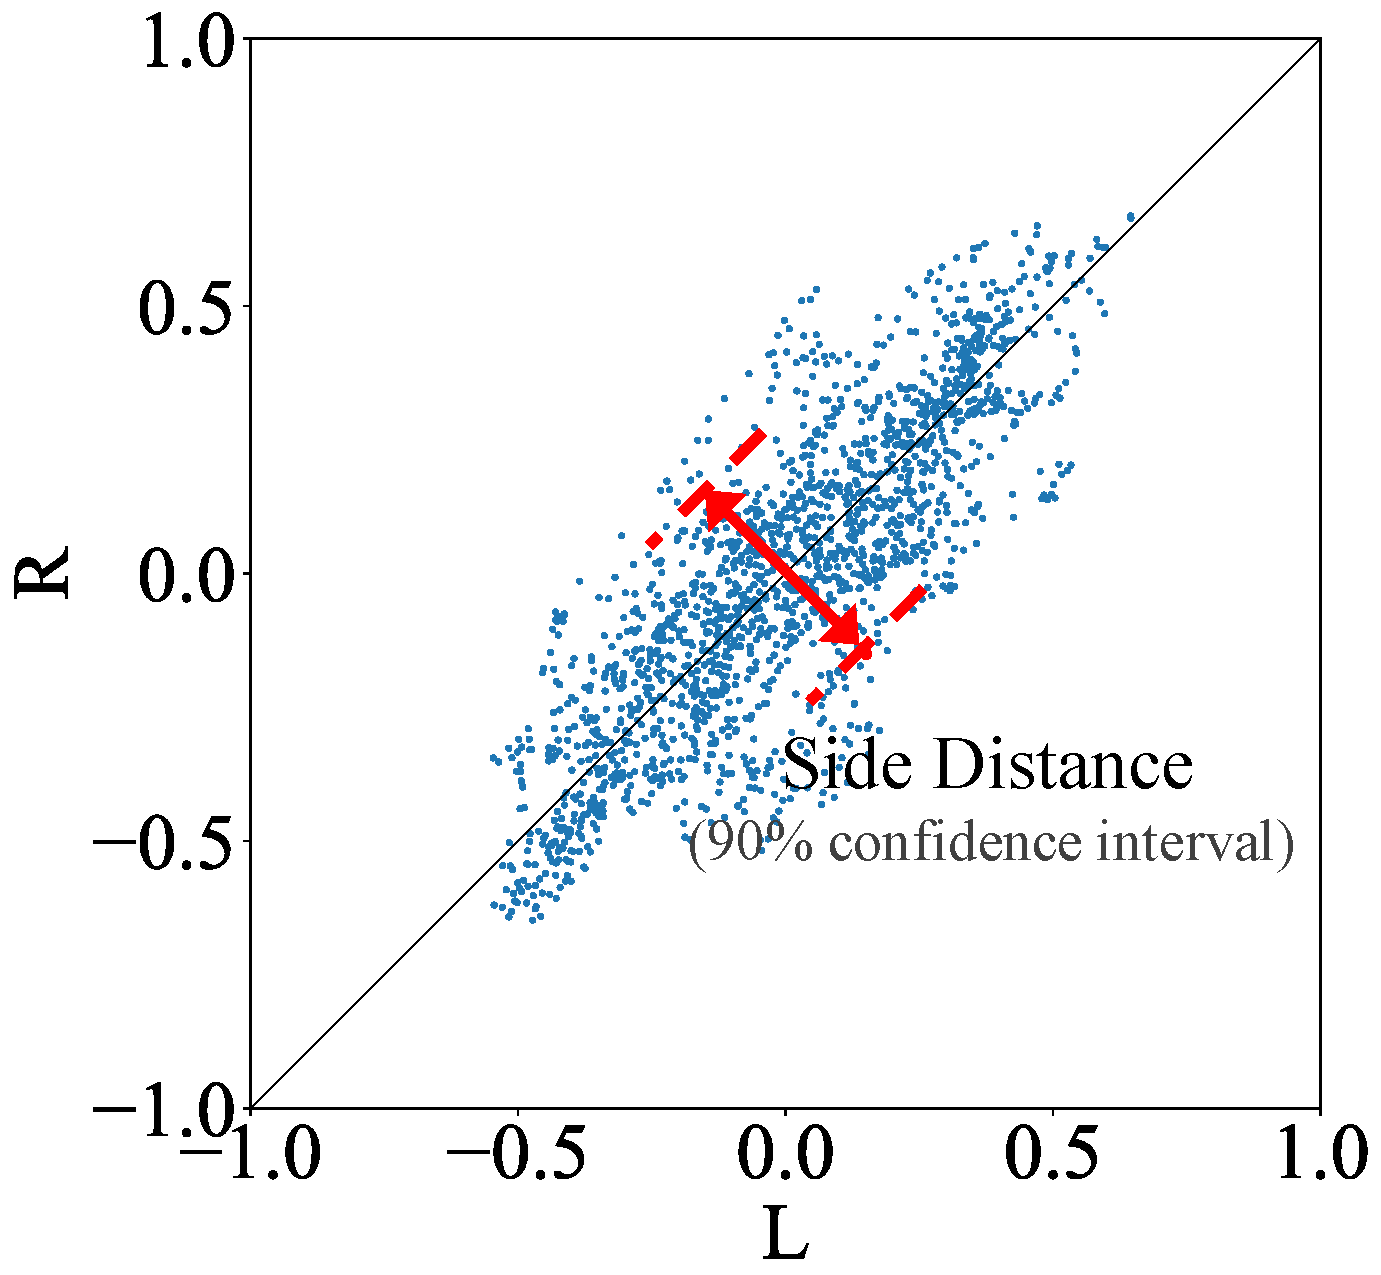
\includegraphics[width=0.4\linewidth]{assets/figures/scatter_38.pdf}
    \end{block}
\end{frame}

\begin{frame}{Features of stereo audio}
    \begin{block}{Short-time Side Distance (STSD)}
        \begin{itemize}
            \item Although side distance is an indicator of how wide the given stereo audio is spread in the auditory space, it cannot express the change of the stereo image over time.
            \item We introduce the concept of STSD to capture the characteristics of the stereo image over time.
            \item Sequence of side distance of a windowed signal\\
            $\rightarrow$ $STFT(y(t)) = D_{side}(y(\tau)w(t))$
        \end{itemize}
        \bigskip
        \centering
        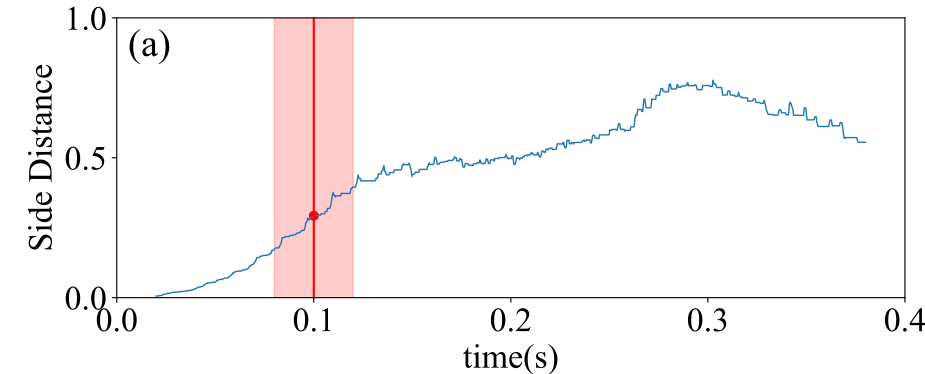
\includegraphics[width=0.5\textwidth]{Presentation/figures/stsd_ppt.png}
    \end{block}
\end{frame}

\begin{frame}{Evaluation Metrics}
    \begin{block}{Distance between two STSDs}
        \begin{itemize}
            \item Earth Mover's Distance\\
            $EMD(s_1, s_2) = \min_{\phi: s_1\to s_2} \sum_{x\in s_1} \|x-\phi(x)\|_2$\\
            (where $\phi$ is a bijection between $s_1, s_2$)
        \end{itemize}
    \end{block}
    \begin{block}{Metric between two sets}
        \begin{itemize}
            \item Minimum Matching Distance\\
            $MMD(S_g, S_r) = \frac{1}{|S_r|}\sum_{Y\in S_r} \min_{X\in S_g}D(X,Y)$
            \item Coverage\\
            $COV(S_g, S_r) = \frac{|\{\arg\min_{Y \in S_r} D(X,Y) | X \in S_g \}|}{|S_r|}$
            \item 1-Nearest Neighbor Accuracy\\
            $1-NNA(S_g, S_r) = \frac{\sum_{X\in S_g} \mathbbm{1}[N_X \in S_g] +  \sum_{Y\in S_r} \mathbbm{1}[N_Y \in S_r]}{|S_g|+|S_r|}$
        \end{itemize}
    \end{block}
\end{frame}
\subsection{Experimental Results}
\begin{frame}{Experiment setup}
    \begin{itemize}
        \item GANSynth: Train with our training set that composed of mel-spec and IF produced by LR channels.
        \bigskip
        \bigskip
        \item Proposed approach: Train with our training set that composed of mel-spec and IF with reparameterized MS channels.
    \end{itemize}
\end{frame}

\begin{frame}{Quantitative results}
    \begin{itemize}
        \item Better results on every evaluation metrics (COV, MMD, 1-NNA)
    \end{itemize}
    \bigskip
    \bigskip
    \centering
    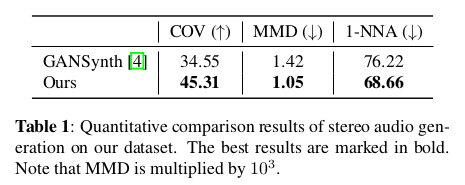
\includegraphics[width=0.7\textwidth]{Presentation/figures/result_table.png}
\end{frame}

\begin{frame}{Qualitative results}
    
\end{frame}